\chapter{Radial Basis Function Neural Network}
\label{chapter:rbf}
\section{簡介}
\label{sec:rbf_introduction}
Radial Basis Function Function(簡稱RBF)Network Work,圖\ref{fig:rbf_network}爲它的網路架構圖,其中有三層網路,分別爲輸入、隱藏層與輸出層。在介紹這個演算法前我們先來看看圖\ref{fig:percepton_problem},在\ref{fig:percepton_Pa}、\ref{fig:percepton_Pb}情況下,我們都可以利用一條線兩種不同類別分割,但是遇到\ref{fig:percepton_Pc}的情況,卻不能用一條線將兩個類別分割出來,由此可見這就是Single Perceptron缺點。而RBF這個演算法的優勢就在於,可以解決了Single Perceptron與MLP在某些情況下線性不可切割的問題,可以將不可線性分割的資料集轉換到另一個維度如圖\ref{Fig:rbf_transfer}所示,使得轉換過的資料變成可線性分割的問題。
\begin{figure}[htbp]
	\centering
	\centerline{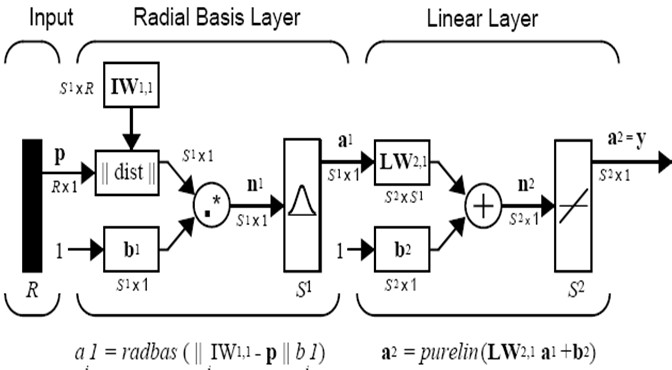
\includegraphics[width=10cm]{pic/rbf_struct.png}}
	\caption{RBF網路架構圖}
	\begin{minipage}{.7\linewidth}
		\footnotesize
		\emph{圖片來源:}取自Function approximation using artificial neural networks
	\end{minipage}
	\label{fig:rbf_network}
\end{figure}

\begin{figure}[!t]
	\begin{center}
		\begin{tabular}{ccccccccccccc}
			\subfigure[]{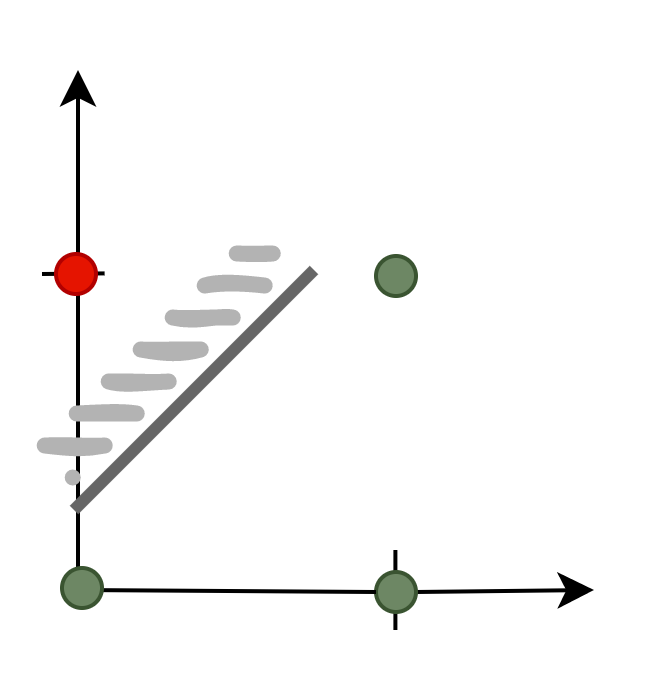
\includegraphics[height=4cm]{./pic/q9iv7T7i.png}\label{fig:percepton_Pa} } \par &
			\subfigure[]{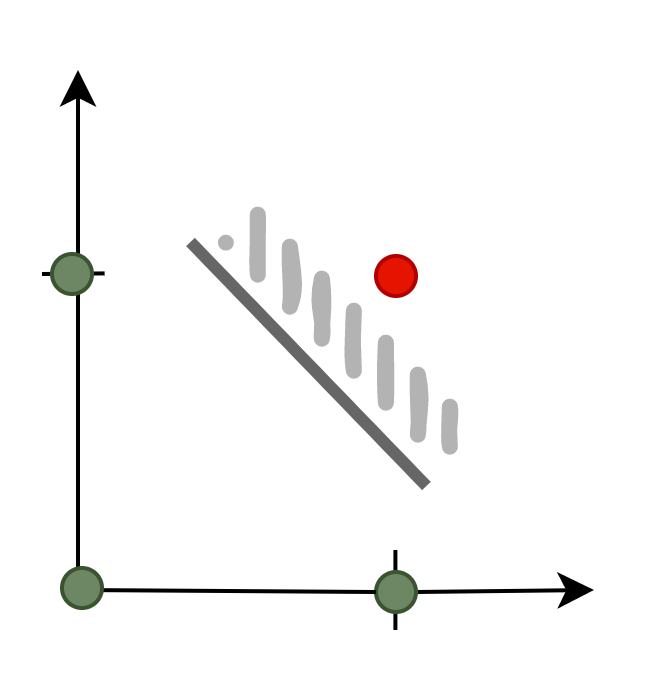
\includegraphics[height=4cm]{./pic/gQvdNdfq.png}\label{fig:percepton_Pb} } \par &
			\subfigure[]{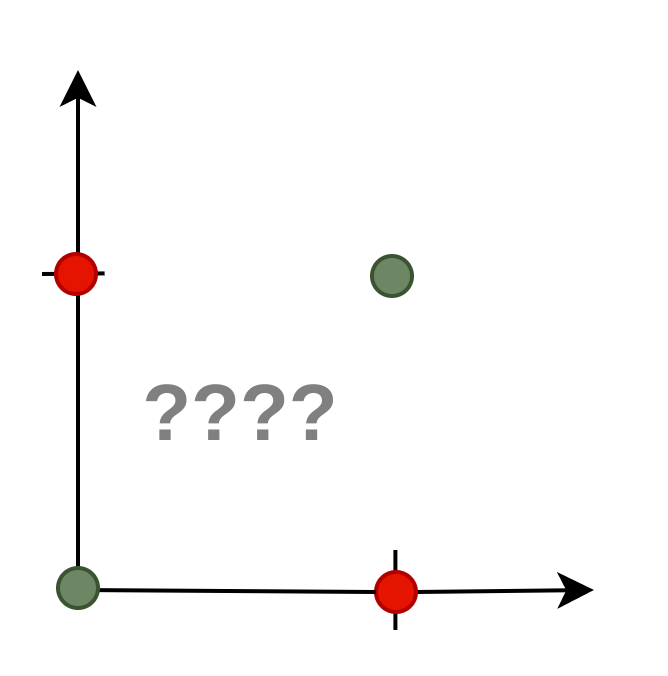
\includegraphics[height=4cm]{./pic/zLfLBK3B.png}\label{fig:percepton_Pc} } \par   \\
		\end{tabular}
		\caption{}
		\label{fig:percepton_problem}
	\end{center}
\end{figure}


%figure3
\begin{figure}[htbp!]
	\centering
	\subfigure[未轉換過的原資料]{
		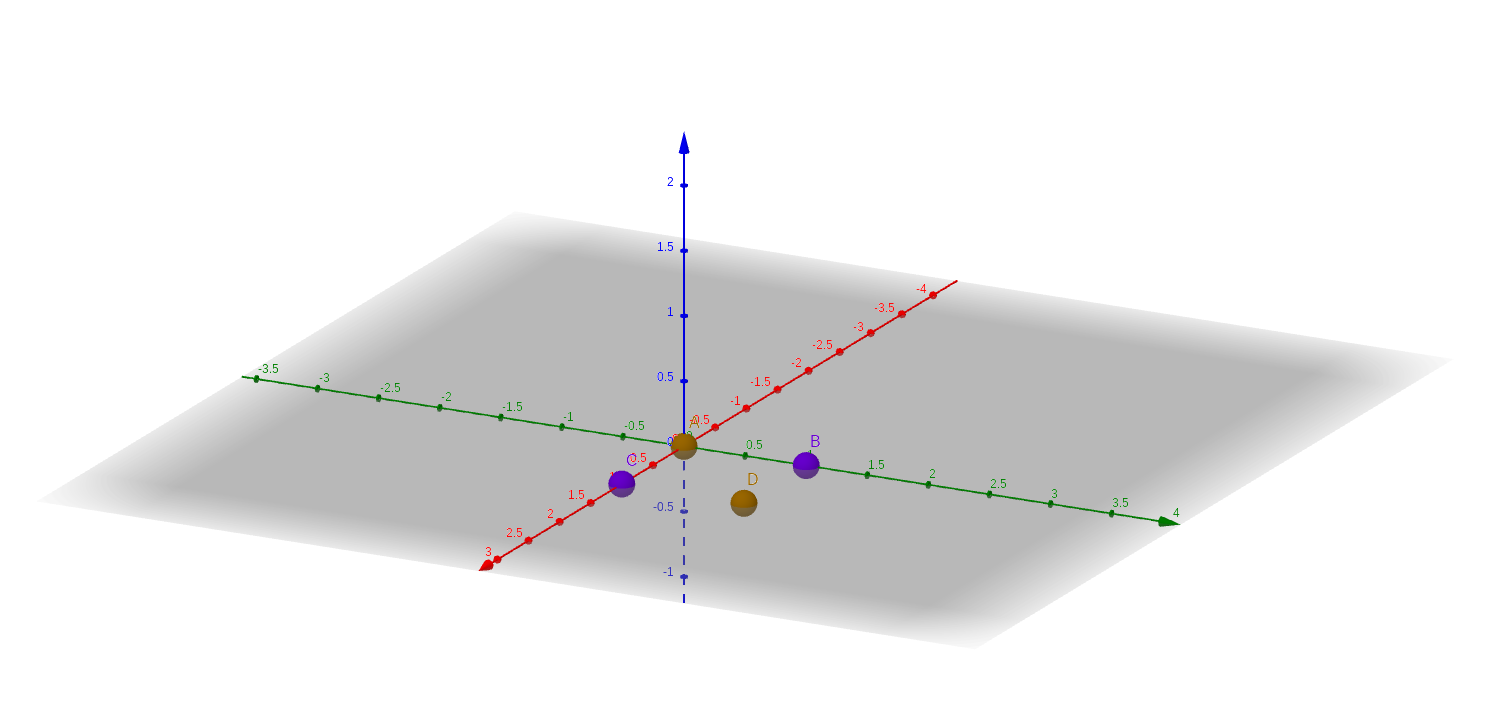
\includegraphics[width=10cm]{pic/Mxrc4anf.png}
		%\caption{fig1}
	}

	%	\quad
	\subfigure[經過轉換後的資料]{
		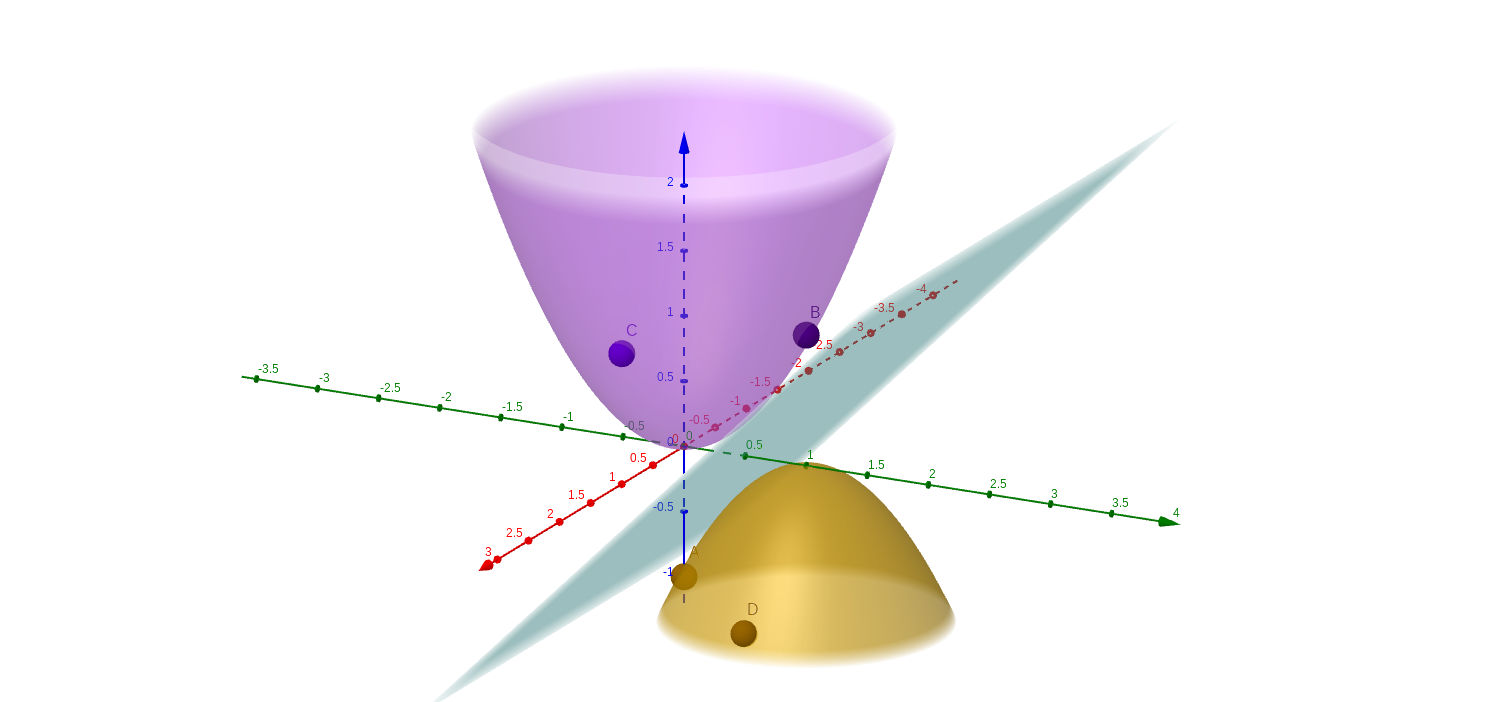
\includegraphics[width=10cm]{pic/JmIpjiQ2.png}
	}

	\caption{資料轉換的示意圖}
	\label{Fig:rbf_transfer}
\end{figure}



\section{Radial Basis Function}
前一小節提到RBF神經網路可以將資料轉換到另一個維度,而這個能將資料轉換到另一個維度的函數就是Hiden Layer中的 \(h(.)\),它也就是Radial Basis Function,以下舉個例子來說明它的運作:

\begin{itemize}
	\item

	      圖\ref{fig:rbf_introduction_not_transfer}為一個一維的資料集,其中有藍色與橘色兩個類別,而我們的任務就是將這兩個類別分開。乍看之下僅用一條線將其分開,幾乎是不可能的任務,但是這也是我們限制在一個維度下才不能將其分離。



	      \begin{figure}[h]
		      \centering
		      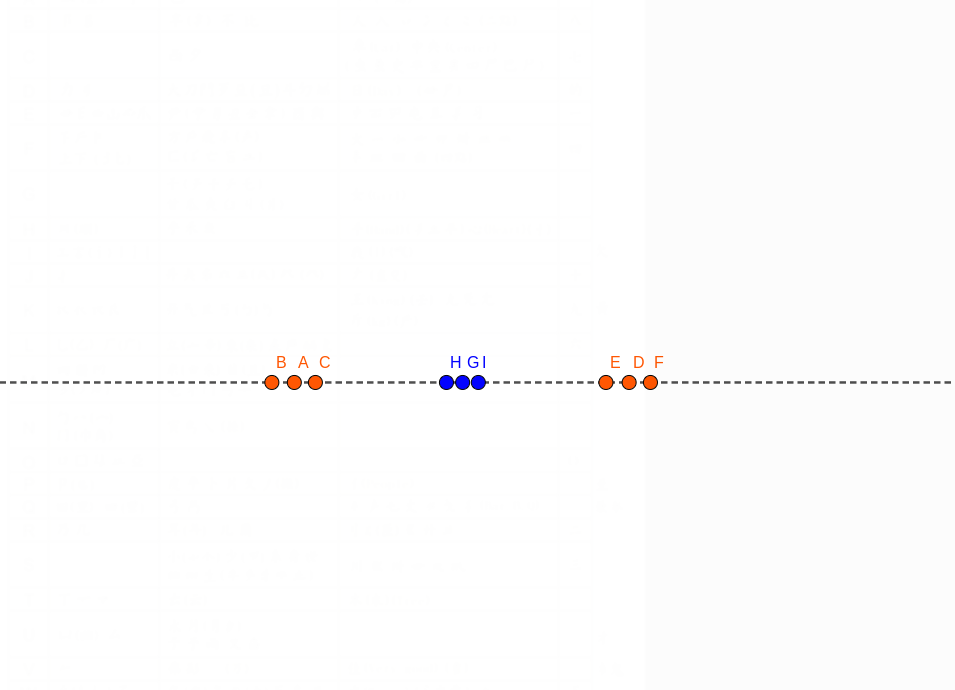
\includegraphics[height=6cm]{./pic/vM4xT9rm.png}
		      \caption{一維資料集}
		      \label{fig:rbf_introduction_not_transfer}
	      \end{figure}

	\item
	      現在我們有一個 \(f(x)\) ,當我們的資料點經過這個函數的轉換,可以發現橘色點都向上移動,而藍色點都向下移動。經過函數轉換的結果後,我們要將這兩個類別進行切割就不難了。

	      \begin{figure}[h]
		      \centering
		      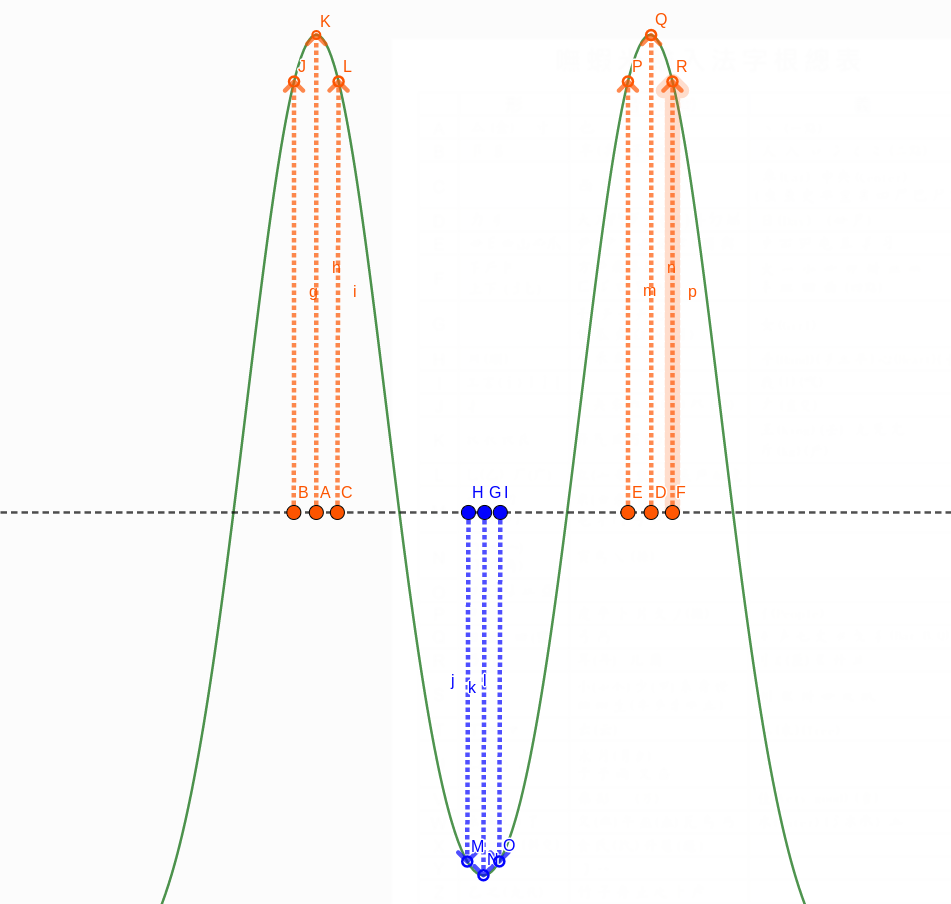
\includegraphics[width=6cm]{./pic/7VM3Lid5.png}
		      \caption{經過 \(f(x)\)轉換的結果 }
		      \label{fig:rbf_with_function}
	      \end{figure}


	\item
	      而這個 \(f(x)\),其實是由3個不同的函數所組成在外加一個常數項所組成的,如圖\ref{fig:lvq_function_assemble}與\ref{eqn:lvq_function}式所示。而其中的 \(h_1(x)\)、\(h_2(x)\)與\(h_3(x)\)就是就是 Radial Basis Function,藉由他們的組成可以將原本的資料集轉換到另一個維度。

	      \begin{equation}
		      \label{eqn:lvq_function}
		      f(x)=w_1h_1(x)+w_2h_2(x)+w_3h_3(x)+b
	      \end{equation}

	      \begin{figure}[h]
		      \centering
		      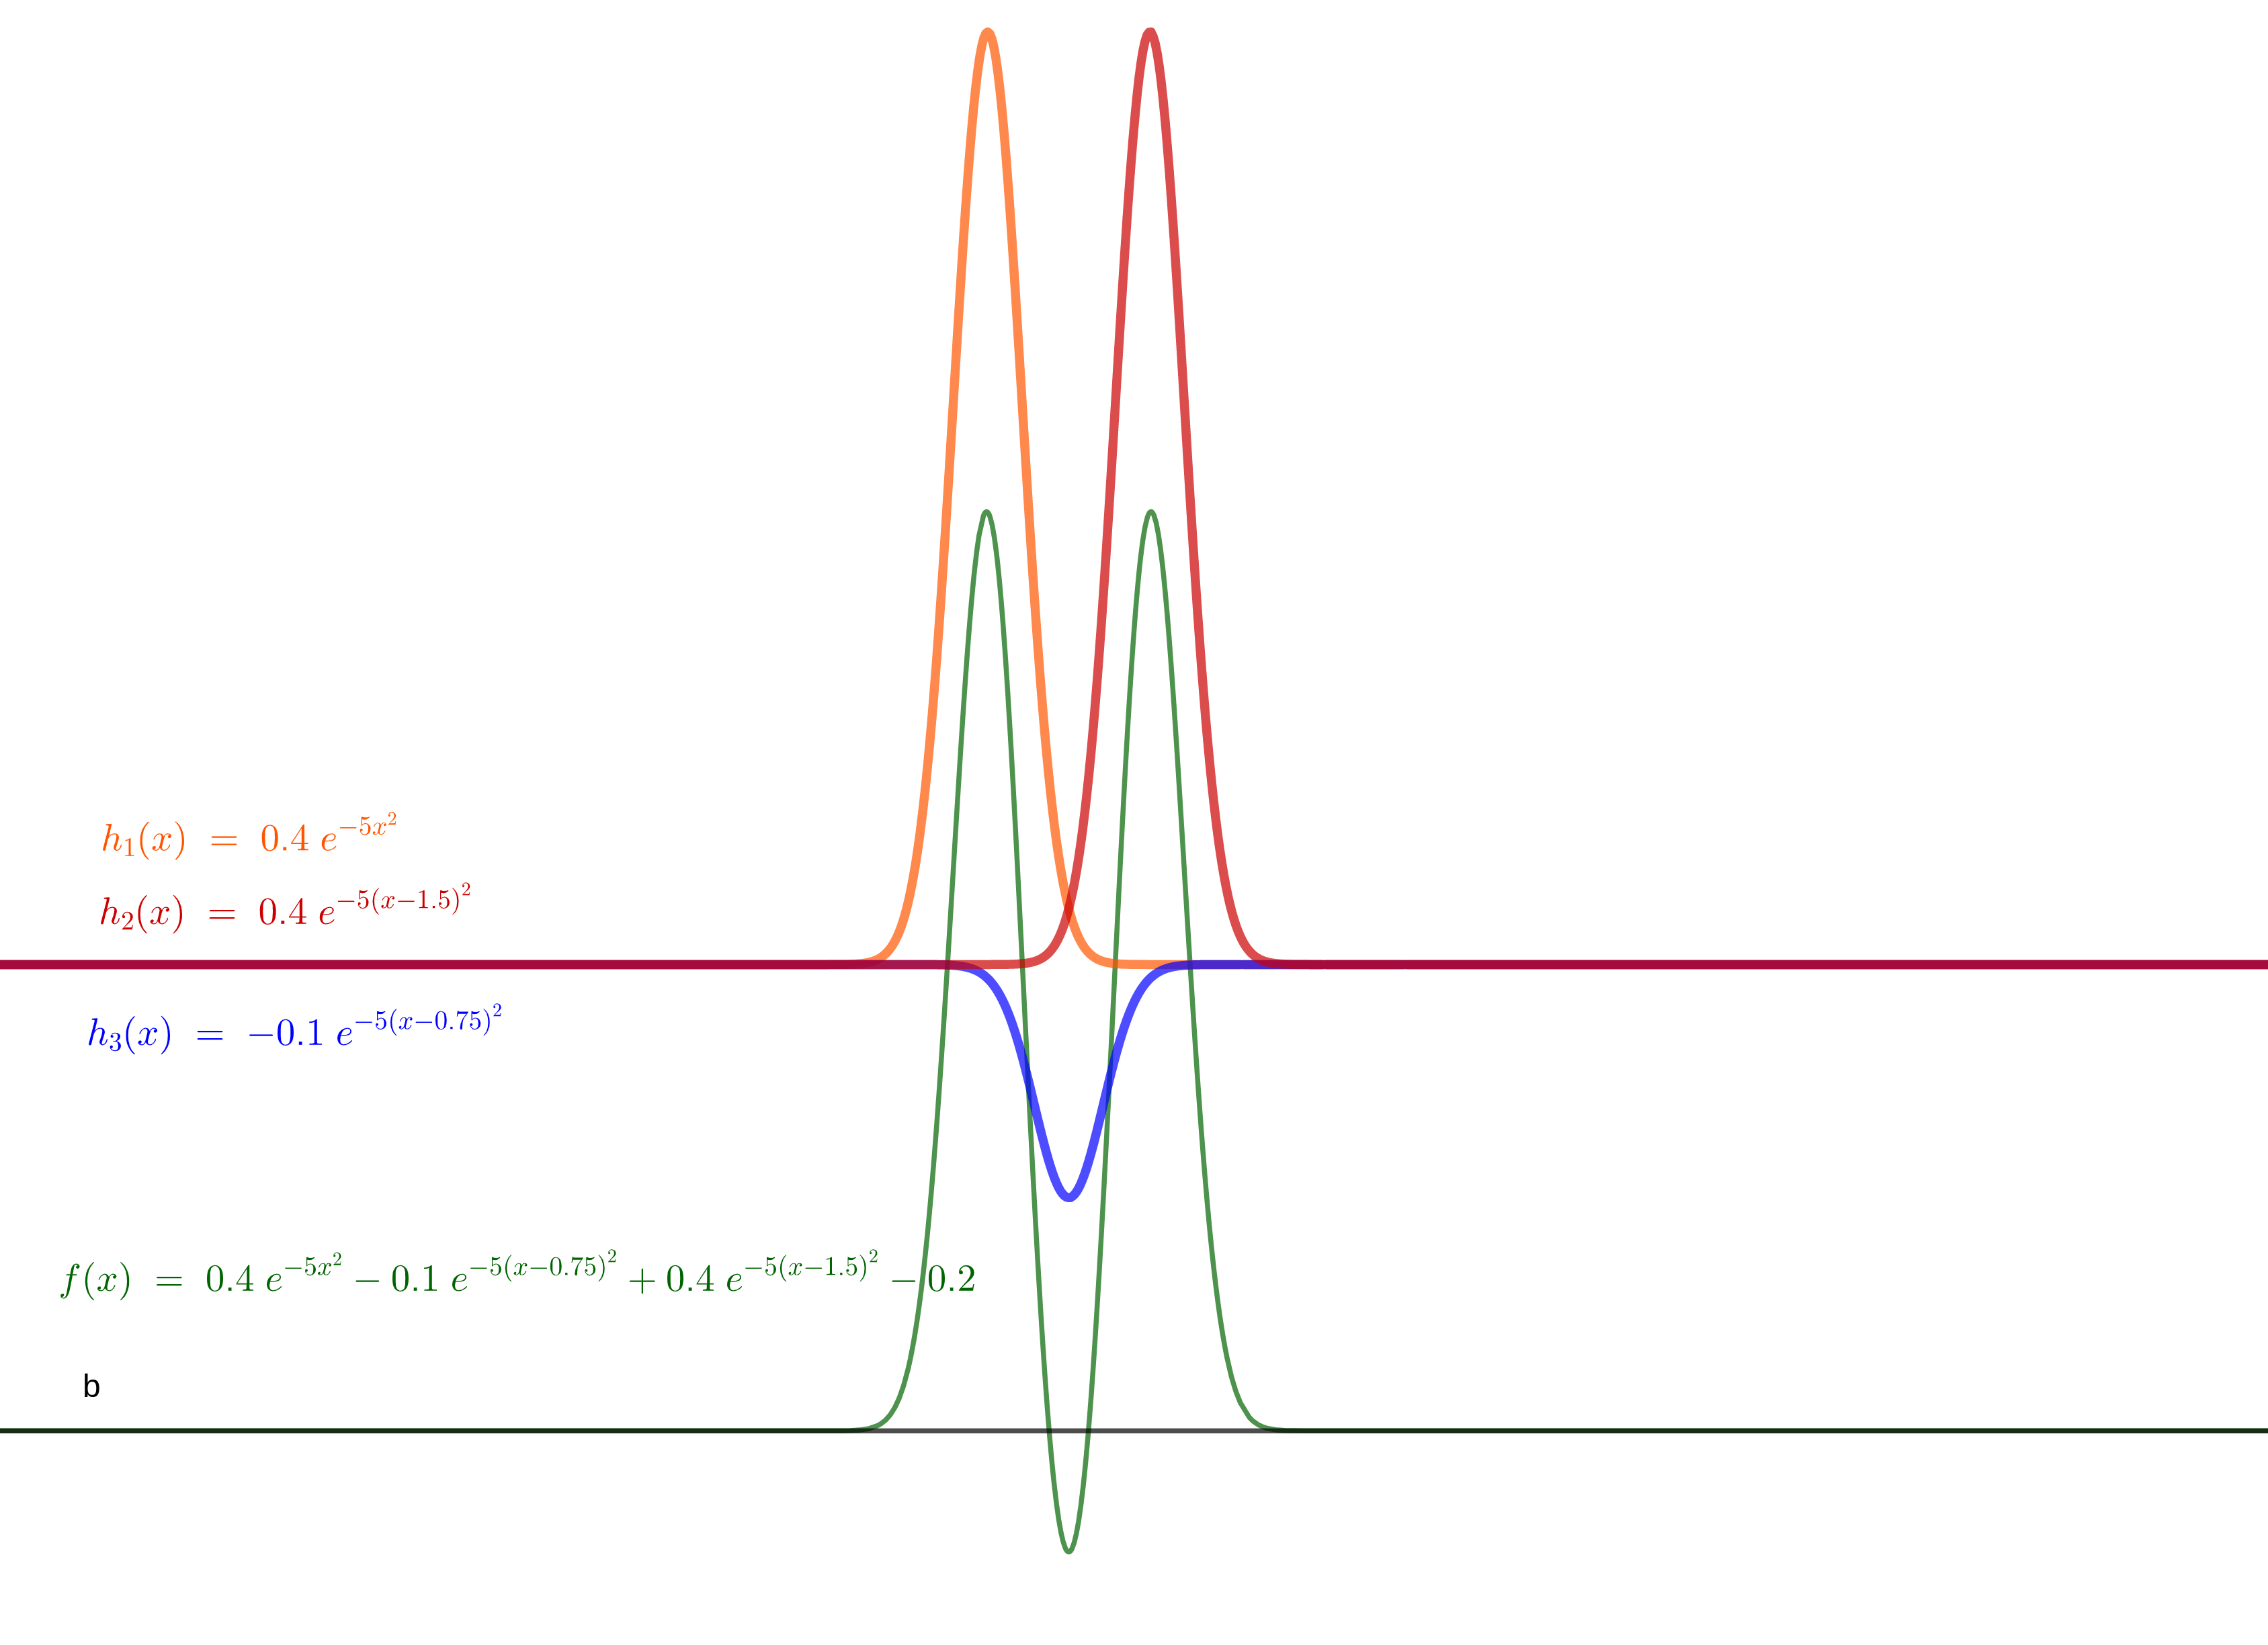
\includegraphics[height=6cm]{./pic/vtYD2no6.png}
		      \caption{\(f(x)\)的組成 }
		      \label{fig:lvq_function_assemble}
	      \end{figure}

	\item
	      Radial Basis Function(徑向基函數),之所以有個「Radial」,其實不難想像,就是跟中心點的距離有關係,所以通常這個函數會設定一個中心點,並將其他點與這個中心點的距離代入計算輸出結果。
	      式 \ref{eqn:radial_basis_function}與圖\ref{fig:radial_basis_function},爲一個中心點為1的高斯函數。
	      從圖中也能發現,離中心點越近可以得到越大值,代表與中心點越相關。反之離中心點越遠所得到的值就越小,代表與中心點越不相關。

	      \begin{equation}
		      \label{eqn:radial_basis_function}
		      h(x)= e^{-|1-x|^2}
	      \end{equation}

	      \begin{figure}[H]
		      \centering
		      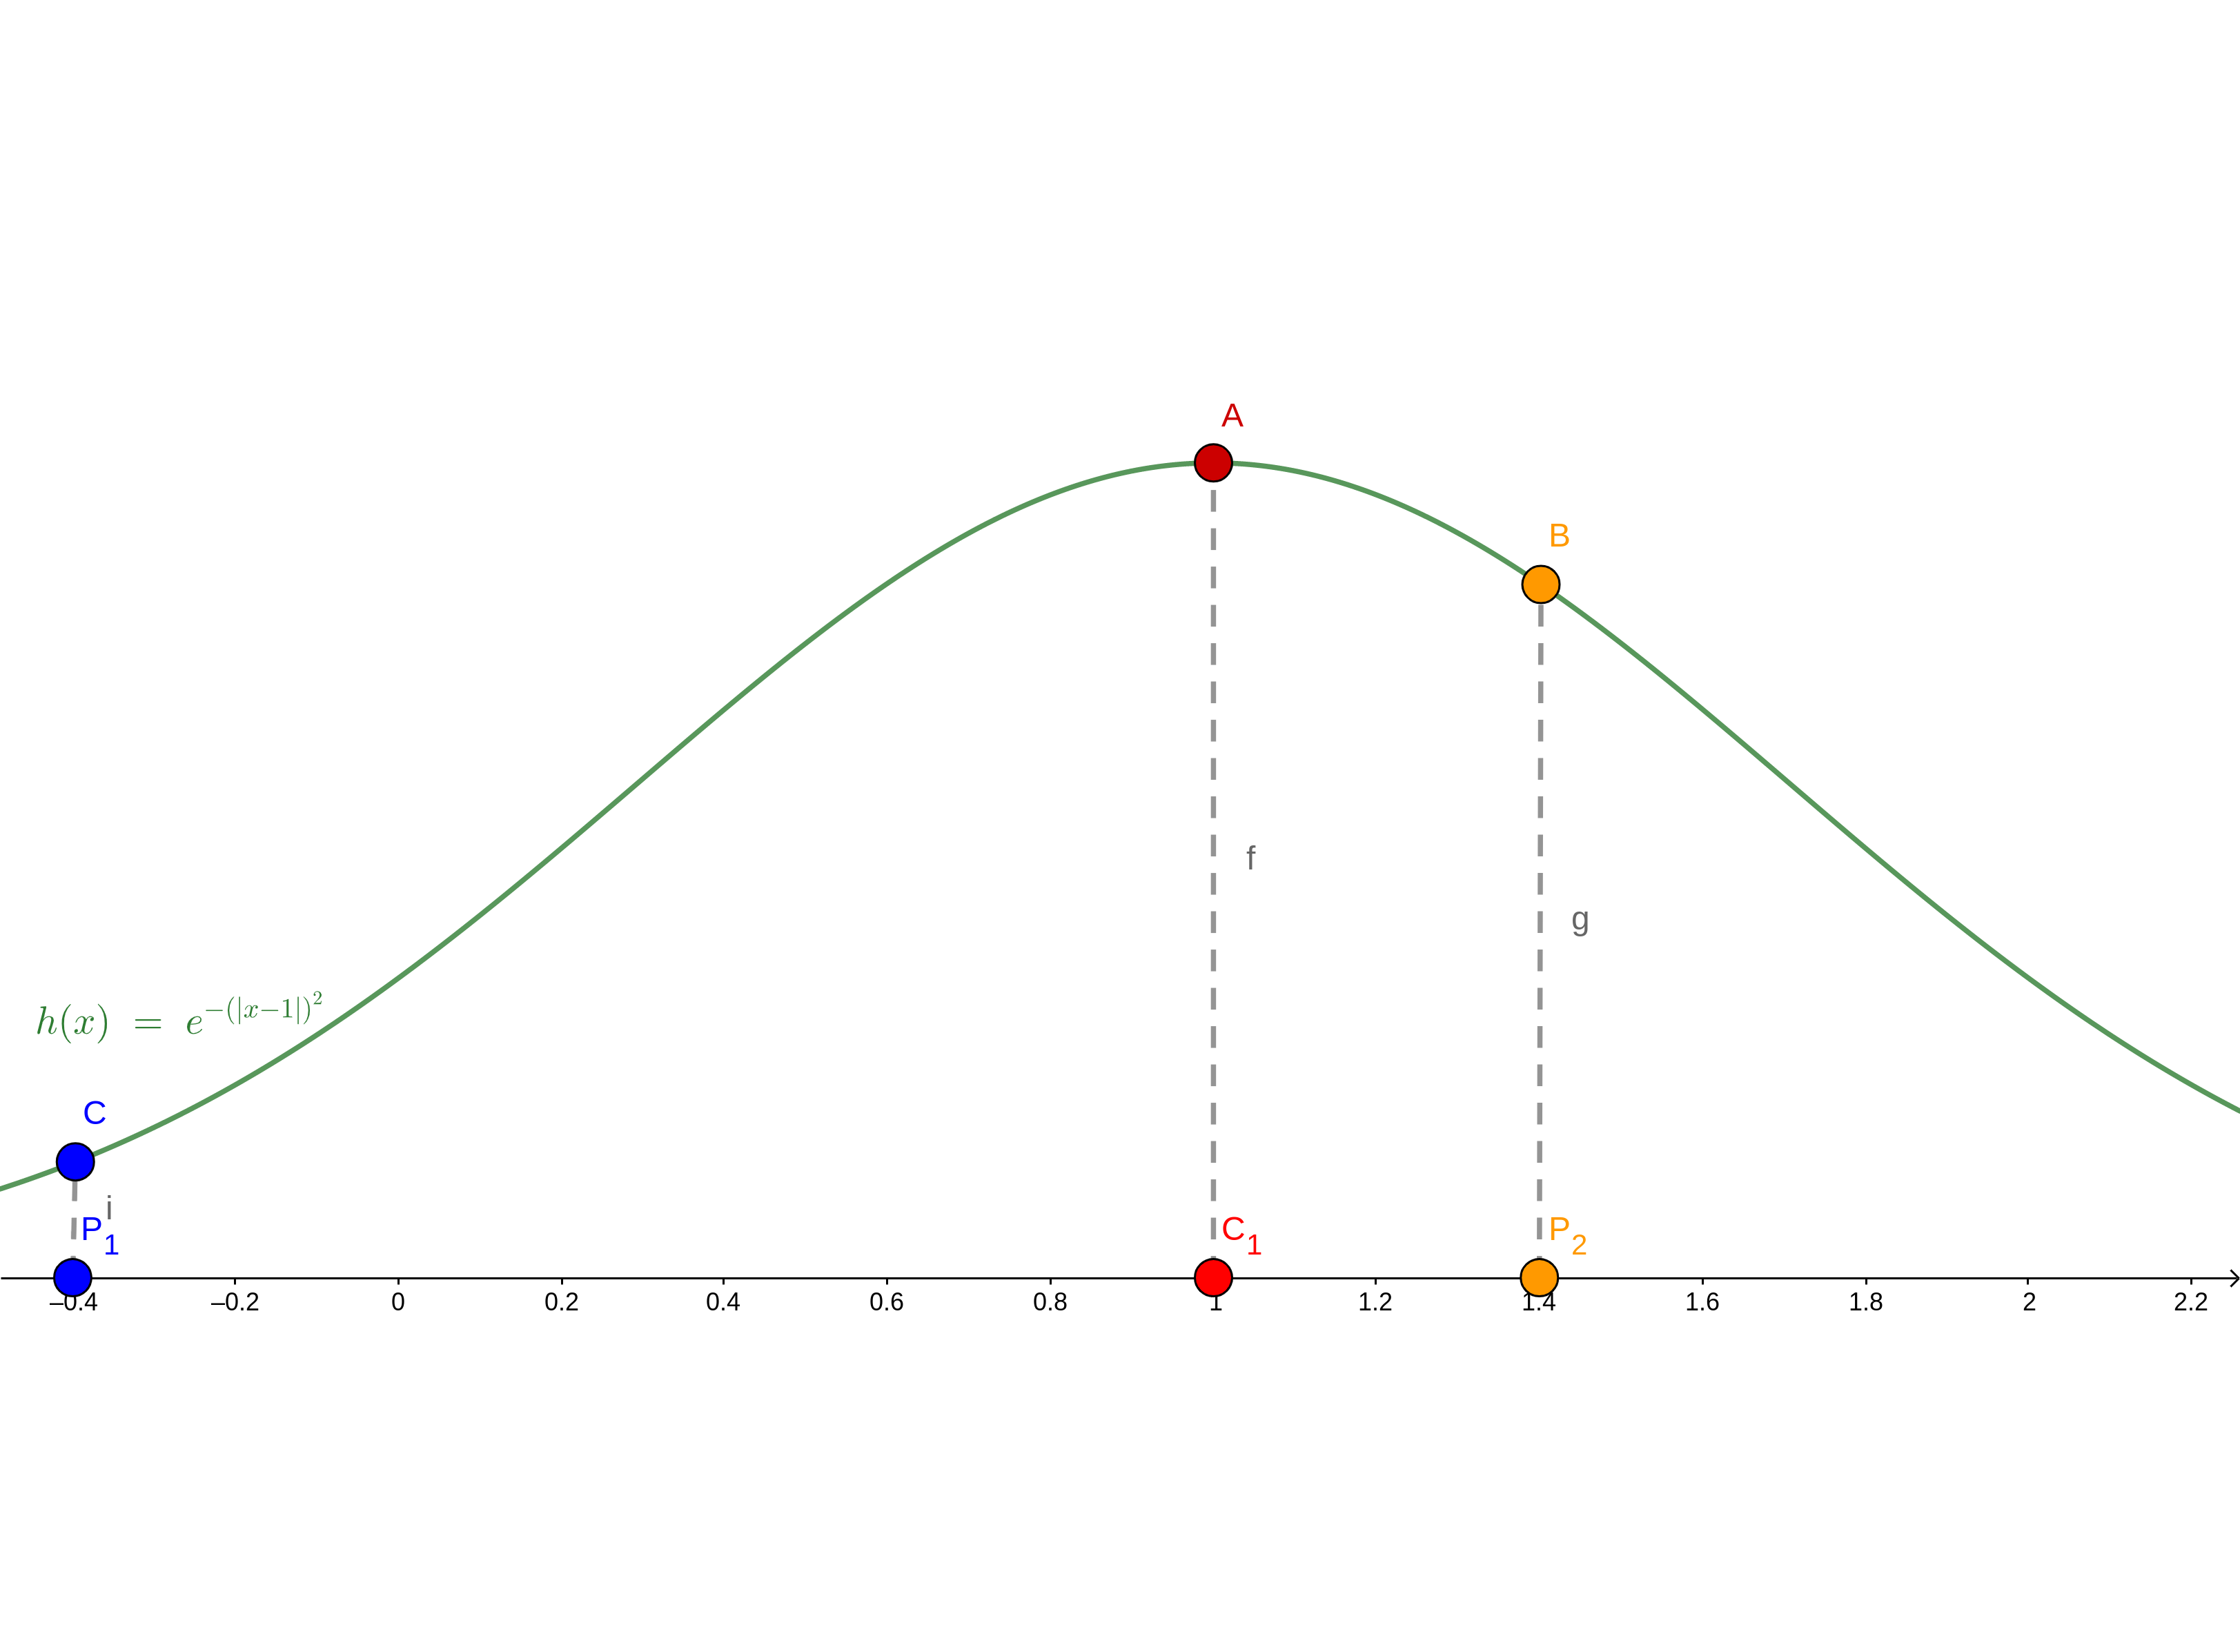
\includegraphics[height=6cm]{./pic/w0KFLczH.png}
		      \caption{}
		      \label{fig:radial_basis_function}
	      \end{figure}

\end{itemize}

當然Rail Basis Function有很多種,常見的如下表所示:
\\

\begin{table}[h!]
	\centering
	\label{tab:rbf_table}
	\begin{tabular}{ccc}
\toprule
  & RBF的名字 & 方程式 (\(r = ||\mathbf{C-X_i}||\) )   \\ 
\midrule
  & Gaussian Function  & \(h(r) = e^{-\varepsilon r}\)      \\ \\ 
  & Linear radial Function  & \(h(r) = r\)      \\ \\
  & Multiquadric   & \(h(r) = \sqrt{1+(\varepsilon r)^2}\)       \\ \\
  & Inverse quadric  &  \(h(r) = \frac{1}{1+(\varepsilon r)^2}\)     \\ \\ 
  & Inverse Multiquadric  &  \(h(r) = \frac{1}{\sqrt{1+(\varepsilon r)^2}}\)     \\
\bottomrule
\end{tabular}

	\caption{常見的Radial Basis Function}
\end{table}







%要被單行註解的文字。


\section{演算法參數定義與流程}




\subsection{參數定義}
\begin{itemize}
	\item
	      輸入向量,\(\mathbf{x} = (x_1,x_2,x_3,....,x_R)\),爲資料集中的其中一筆資料,輸入向量的數量 \(R\) 爲資料的特徵數量。
	      %
	\item
		Radial Basis Layer權重,\(\mathbf{W^1} = [\mathbf{c_1,c_2,...,c_j,...c_{S_1}}]^T\),爲一個 \(S_1 \times R \)的矩陣,也就是前一節所介紹 Radial Basis Function中心點的集合,這邊的 \(S_1\)代表中心點的數量,而 \(\mathbf{c_j}\)為其中一個中心點 。
	      %
	\item
		Radial Basis Function, 定義為\(\{h_1(.), h_2(.),...,h_j(.),....h_{S_1}(.) \}\)  
	\item
		輸出層權重, \(\mathbf{W^2}= [\mathbf{w_1,w_2,...,w_j,...,w_{S_2}}]^T\),為一個 \(S_2 \times S_1\) 的矩陣,這邊的 \(S_2\)代表輸出的類別數 。偏移向量為, \(\mathbf{b^2}=(b_1,b_2,....b_{S_2})\)。 
	      %
\end{itemize}

\section {演算法參數定義與流程}
研究方法與論文架構,研究方法與論文架構,研究方法與論文架構,
研究方法與論文架構,研究方法與論文架構,研究方法與論文架構,
研究方法與論文架構,研究方法與論文架構,研究方法與論文架構,
研究方法與論文架構。

\begin{itemize}
	\item
	      項目一。
	      %
	\item
	      項目二。
	      %
	\item
	      項目三。
	      %
	\item
	      項目四。
\end{itemize}

流程圖如\ref{fig:ResearchFlowChart}。
\begin{figure}[htbp]
	\centering
	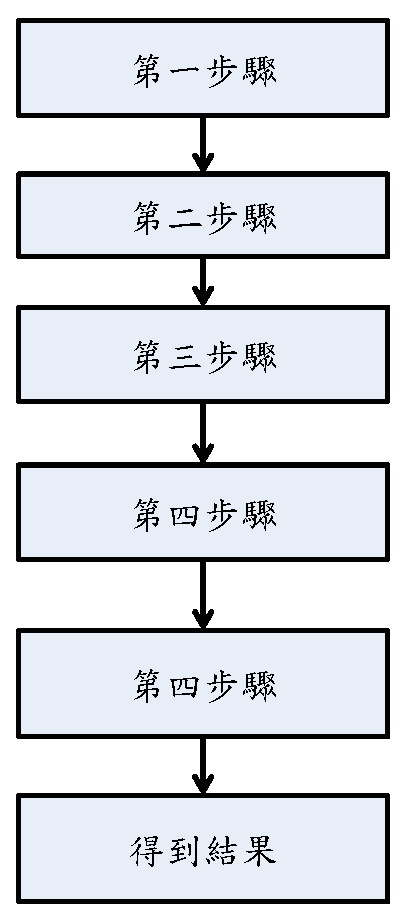
\includegraphics[height=8cm]{graphs/introduction/ResearchFlowChart.eps}
	\caption{研究進行流程圖}
	\label{fig:ResearchFlowChart}
\end{figure}
